\documentclass[aspectratio=169,12pt,spanish]{beamer}
\usepackage[T1]{fontenc}
\usepackage[spanish]{babel}

\usepackage{wrapfig}

%\usepackage{multicol}
%\usepackage{mathtools}

\usepackage[normalem]{ulem}

\usepackage{pgf,tikz}
\usetikzlibrary{matrix}
\usetikzlibrary{arrows}

%\usepackage{wrapfig}
\mode<presentation>
\usefonttheme{professionalfonts}
\usetheme{Darmstadt}
\usecolortheme{orchid}
\useoutertheme{default}
\setbeamertemplate{headline}{}

\newcounter{savedenum}
\newcommand*{\saveenum}{\setcounter{savedenum}{\theenumi}}
\newcommand*{\resume}{\setcounter{enumi}{\thesavedenum}}

\renewcommand{\baselinestretch}{1.1}

%gets rid of bottom navigation bars
\setbeamertemplate{footline}[page number]

%gets rid of navigation symbols
\setbeamertemplate{navigation symbols}{}

%\frameframe{none} % No default frame

%\setlength{\framewidth}{8.7in} \setlength{\frameheight}{7.2in}

\parindent 0pt
\setlength{\parskip} {1ex plus 0.5ex minus 0.2ex}


\usepackage[bbgreekl]{mathbbol}
\usepackage{amssymb, amsthm, amsmath}
\usepackage{bm}

\newtheorem{ejercicio}{Ejercicio}
\newtheorem{proposition}[theorem]{Proposición}

\DeclareSymbolFontAlphabet{\mathbb}{AMSb}
\DeclareSymbolFontAlphabet{\mathbbl}{bbold}

\usepackage{multicol}
\usepackage{colortbl}
\usepackage{lmodern}
\usepackage{tabularx}
\usepackage{multirow}
\usepackage{stmaryrd}
\usepackage{color}
\usepackage{graphicx}
\usepackage{hyperref}

\graphicspath{ {../../images} }
\usepackage{listings}
\lstset{
  basicstyle=\ttfamily,
  columns=fullflexible,
}

\usepackage{url}
\usepackage{multicol}
\usepackage{dsfont}

% Bold symbols for vectors and matrices
\newcommand{\xstar}{\bm{x}^{\star}}
\newcommand{\alphab}{\bm{\alpha}}
\newcommand{\ab}{\bm{a}}
\newcommand{\bb}{\bm{b}}
\newcommand{\cb}{\bm{c}}
\newcommand{\db}{\bm{d}}
\newcommand{\eb}{\bm{e}}
\newcommand{\gb}{\bm{g}}
\newcommand{\mb}{\bm{m}}
\newcommand{\pb}{\bm{p}}
\newcommand{\qb}{\bm{q}}
\newcommand{\rb}{\bm{r}}
\newcommand{\ssb}{\bm{s}}
\newcommand{\ub}{\bm{u}}
\newcommand{\vb}{\bm{v}}
\newcommand{\wb}{\bm{w}}
\newcommand{\xb}{\bm{x}}
\newcommand{\yb}{\bm{y}}
\newcommand{\zb}{\bm{z}}

\newcommand{\Ab}{\bm{A}}
\newcommand{\Bb}{\bm{B}}
\newcommand{\Cb}{\bm{C}}
\newcommand{\Db}{\bm{D}}
\newcommand{\Eb}{\bm{E}}
\newcommand{\Fb}{\bm{F}}
\newcommand{\Gb}{\bm{G}}
\newcommand{\Hb}{\bm{H}}
\newcommand{\Ib}{\bm{I}}
\newcommand{\Id}{\bm{I}}
\newcommand{\Kb}{\bm{K}}
\newcommand{\Lb}{\bm{L}}
\newcommand{\Mb}{\bm{M}}
\newcommand{\Pb}{\bm{P}}
\newcommand{\Qb}{\bm{Q}}
\newcommand{\Rb}{\bm{R}}
\newcommand{\Sb}{\bm{S}}
\newcommand{\Tb}{\bm{T}}
\newcommand{\Ub}{\bm{U}}
\newcommand{\Vb}{\bm{V}}
\newcommand{\Wb}{\bm{W}}
\newcommand{\Xb}{\bm{X}}
\newcommand{\Yb}{\bm{Y}}
\newcommand{\Zb}{\bm{Z}}
\newcommand{\Lambdab}{\bm{\Lambda}}
\newcommand{\cero}{\bm{0}}

% Rings and fields
\newcommand{\A}{\mathbb{A}}
\newcommand{\Z}{\mathbb{Z}}
\newcommand{\Q}{\mathbb{Q}}
\newcommand{\C}{\mathbb{C}}
\newcommand{\R}{\mathbb{R}}
\newcommand{\K}{\mathbb{K}}
\newcommand{\N}{\mathbb{N}}

\newcommand{\borel}{{\mathcal B}}
\newcommand{\pmom}{{\rho_{\text{mom}}}}
\newcommand{\MX}{{\mathcal{M}(X)}}


% Inner product
\newcommand{\innerl}[2]{\langle #1, #2 \rangle}
\newcommand{\inner}[2]{#1 \boldsymbol{\cdot} #2}
\newcommand{\innerTrace}[2]{#1 \bullet #2}

% Symmetric and positive definite matrices
\newcommand{\Splusplusn}{{\mathcal S_{++}^n}}
\newcommand{\Splusn}{{\mathcal S_+^n}}
\newcommand{\Splus}{{\mathcal S_+}}
\newcommand{\Sym}{{\mathcal S}}
\newcommand{\Symn}{{\mathcal S^n}}

% Cones
\newcommand\CC{\mathcal{C}}
\DeclareMathOperator{\cone}{cono}
\DeclareMathOperator{\conv}{conv}
\DeclareMathOperator{\supp}{supp}


% Spectrahedron
\newcommand{\eLL}{{\mathcal L}}

% Matrices and vectors over R or C
\newcommand{\Rnn}{\R^{n\times n}}
\newcommand{\Cnn}{\C^{n\times n}}
\newcommand{\Rn}{\R^{n}}
\newcommand{\Rm}{\R^{m}}


% Math operators
\DeclareMathOperator{\Tr}{Tr}
\DeclareMathOperator{\tr}{Tr}
\DeclareMathOperator{\interior}{int}
\DeclareMathOperator{\rank}{rank}
\DeclareMathOperator{\diag}{diag}

\newcommand\one{\mathds{1}} 

\pagestyle{empty}

\begin{document}

%------------------------------------------------------------------

\begin{frame}

 \begin{center}

\Large\textbf{Optimización Semidefinida} \\
\large\textbf{Clase 08 - Aplicación: max cut}
%\vspace{0.5cm}

% \textit{Santiago Laplagne} \\
%slaplagn@dm.uba.ar \\


%\vspace{0.5cm}
%{\small Trabajo en progreso en conjunto con \emph{Jose Capco} (Universit\"at Innsbruck) y \emph{Claus Scheiderer} %(Universit\"at Konstanz).} \\

\vspace{1cm}
 Segundo Cuatrimestre 2021
 \\
 {\small Facultad de Ciencias Exactas y Naturales, UBA}
 \end{center}

\end{frame}



%------------------------------------------------------------------

\begin{frame}
\frametitle{El problema max cut}

Consideramos un grafo no-dirigido $G = (N, E)$, donde $N$ es el conjunto de nodos y $E \subset N \times N$ es el conjunto de aristas. Suponemos $N = \{1, \dots, n\}$.

Definimos una matriz de costos no-negativos $W = (w_{ij}) \subset \R_{\ge 0}^{n \times n}$.

Podemos suponer que el grafo es completo, es decir que todos los nodos son adyacentes entre sí, tomando $w_{ij} = 0$ para todas las no-aristas $ij$; definimos también $w_{ii} = 0$ para todo $i$.

Como el grafo es no-dirigido, $W$ resulta una matriz simétrica.

\end{frame}

%------------------------------------------------------------------

\begin{frame}
\frametitle{Ejemplo}
\begin{minipage}[t]{0.4\textwidth}
Consideramos el siguiente grafo con los costos indicados.
\begin{center}
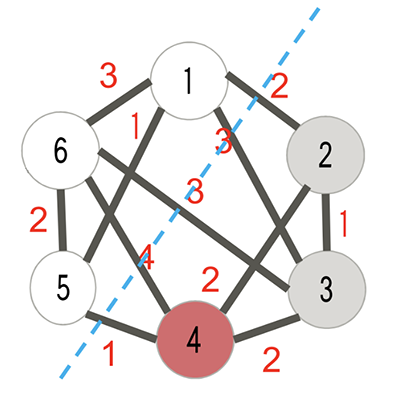
\includegraphics[scale=0.6]{maxcut-example3.png}
\end{center}
\end{minipage}
\hspace{1cm}
\begin{minipage}[t]{0.4\textwidth}
La matriz de costos es
$$
\Wb = \begin{pmatrix}
0 & 2 & 3 & 0 & 1 & 3 \\
2 & 0 & 1 & 2 & 0 & 0 \\
3 & 1 & 0 & 2 & 0 & 3 \\
0 & 2 & 2 & 0 & 1 & 4 \\
1 & 0 & 0 & 1 & 0 & 2 \\
3 & 0 & 3 & 4 & 2 & 0
\end{pmatrix}
$$
\end{minipage}

\end{frame}

%------------------------------------------------------------------

\begin{frame}
\frametitle{Motivación}


Para un subconjunto $K \subset N$ de nodos, definimos el corte $\delta(K)$ como el conjunto de todos las aristas desde $K$ al complemento de $K$:
$$
\delta(K) = \{(i,j) \in E : i \in K, j \notin K\}.
$$
Dado un corte $K$ definimos el costo del corte
$$
w(\delta(K)) := \sum_{(i,j) \in \delta(K)} w_{ij}.
$$
Queremos hallar el corte $\delta(K)$ con el mayor costo posible.

\end{frame}

%------------------------------------------------------------------

\begin{frame}
\frametitle{Ejemplo}

En el ejemplo anterior, para considerar el corte de la línea celeste, tomamos $K = \{2, 3, 4\}$.
El costo del corte $\delta(K)$ es
$$
w(\delta(K)) = (2) + (3+3) + (1 + 4) = 13.
$$

Podemos calcularlo sumando los costos de todas las aristas que atraviesa la línea celeste.

\begin{center}
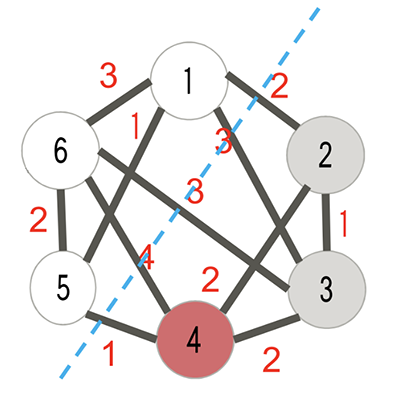
\includegraphics[scale=0.55]{maxcut-example3.png}
\end{center}

\end{frame}

%------------------------------------------------------------------

\begin{frame}
\frametitle{Ejemplo}

En el siguiente grafo de 5 nodos, asignamos costo 1 a todas las aristas dibujadas y costo 0 a las aristas no dibujadas. Tomando $K$ el conjunto de nodos blancos, obtenemos el corte de mayor costo posible.
\begin{center}
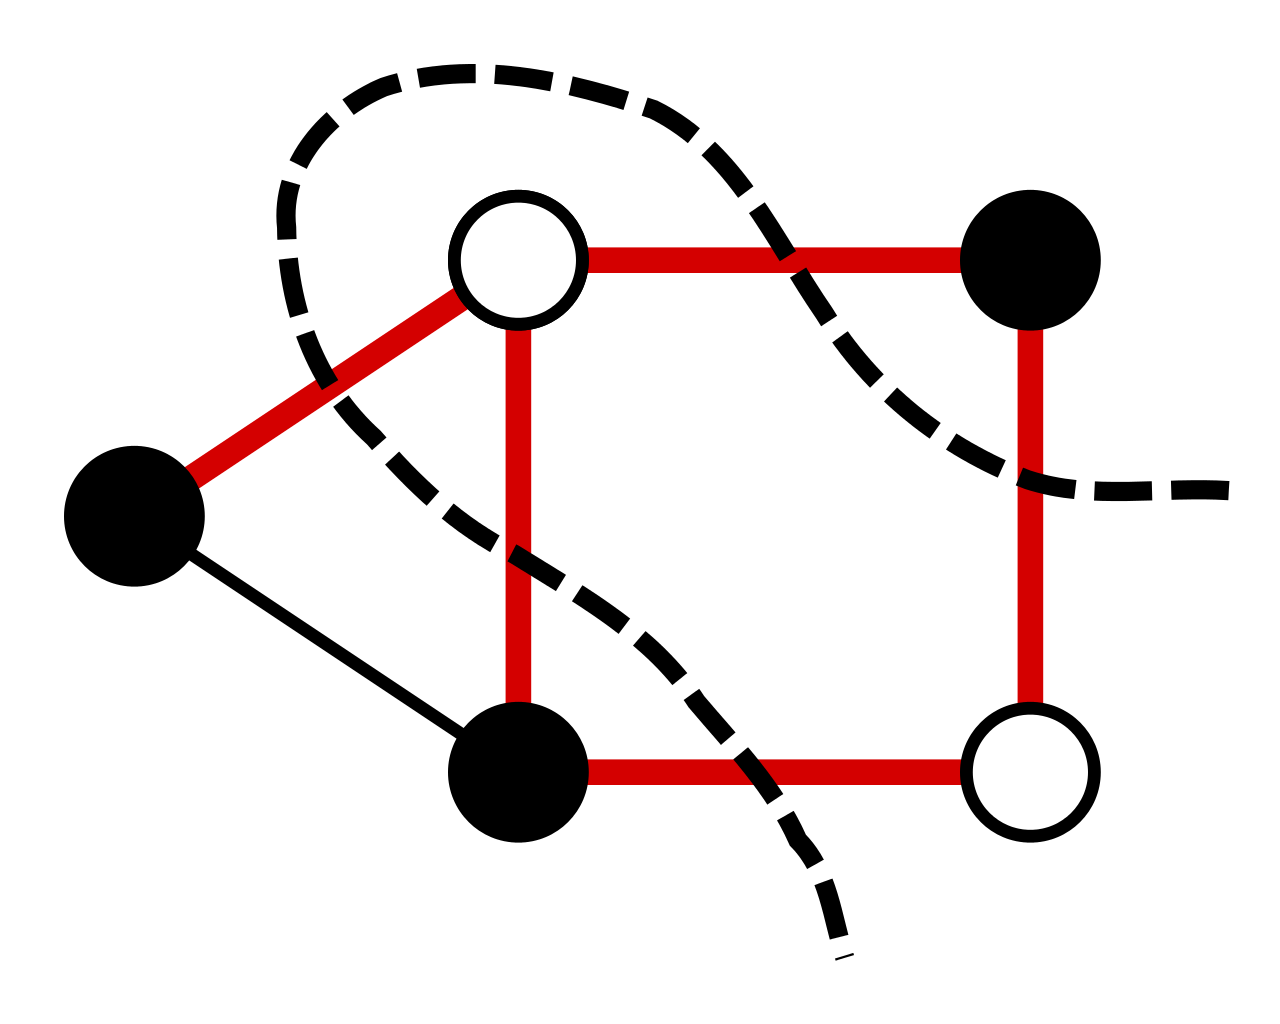
\includegraphics[scale=.15]{1280px-Max-cut.png}
\end{center}



\end{frame}

%------------------------------------------------------------------

\begin{frame}
\frametitle{Ejemplo}

Si consideramos un grafo completo de 4 vértices, con costo 1 en todas las aristas, el costo de un corte queda determinado por la cantidad de nodos en el corte. Obtenemos los siguientes valores:
$$
\delta(K) = \begin{cases}
0 & \text{ si } \#K = 0, \\
3 & \text{ si } \#K = 1, \\
4 & \text{ si } \#K = 2, \\
3 & \text{ si } \#K = 3, \\
0 & \text{ si } \#K = 4. \\
\end{cases}
$$

Por lo tanto, para obtener el corte de mayor costo tomamos un conjunto $K$ de 2 elementos.

\end{frame}

%------------------------------------------------------------------

\begin{frame}
\frametitle{Forma matricial}

Comenzamos formulando el problema en forma matricial. Queremos calcular el costo de un corte mediante un producto de matrices.

Fijamos un corte $K$ y definimos el vector $\xb = (x_1, \dots, x_n) \in \R^n$ por
$$
x_i = \begin{cases}
1 & \text{ si } i \in K \\
-1 &  \text{ si } i \notin K
\end{cases}.
$$
De esta forma, $x_i x_j = -1$ si $(i,j) \in \delta(K)$ y $x_i x_j = 1$ si $(i,j) \notin \delta(K)$, y por lo tanto
$$
1 - x_i x_j = \begin{cases}
2 & \text{ si } (i,j) \in \delta(K), \\
0 &  \text{ si } (i,j) \notin \delta(K).
\end{cases}
$$


\end{frame}

%------------------------------------------------------------------

\begin{frame}
\frametitle{Forma matricial}

Obtenemos
$$
w(\delta(K)) = \sum_{i < j}w_{ij}\frac{1-x_i x_j}{2} = \frac{1}{4}\sum_{i \neq j}w_{ij}(1-x_i x_j).
$$
Como además $w_{ii} = 0$ para todo $i$,
$$
w(\delta(K)) = \frac{1}{4}\sum_i \sum_j w_{ij}(1-x_i x_j) = \left(\frac{1}{4}\sum_i \sum_j w_{ij} \right) - \frac{1}{4} \sum_{i \neq j}w_{ij}(x_i x_j).
$$


\end{frame}

%------------------------------------------------------------------

\begin{frame}
\frametitle{Forma matricial}

Utilizando $x_i^2 = 1$, reescribimos:
$$
\left(\frac{1}{4}\sum_i \sum_j w_{ij} \right) - \sum_{i \neq j}w_{ij}(x_i x_j) = \left(\frac{1}{4}\sum_i \left(\sum_j w_{ij}\right) x_i x_i \right) - \frac{1}{4} \sum_{i \neq j}w_{ij}(x_i x_j).
$$

El primer término corresponde a los productos $x_i x_i$ y el segundo a los productos $x_i x_j$, $i \neq j$.

\end{frame}

%------------------------------------------------------------------

\begin{frame}
\frametitle{Forma matricial}

Definiendo $\Cb \in \R^{n \times n}$ con
\begin{align*}
  c_{ij} &= -w_{ij}/4  \text{ para $i \neq j$}  \\
  c_{ii} &= \sum_j w_{ij}/4 \text{ para todo $i$ },
\end{align*}
obtenemos $w(\delta(K)) = \xb^T \Cb \xb$.

En el ejemplo, obtenemos $\xb^T \Cb \xb = 13$ tomando $\xb = (-1, 1, 1, 1, -1, -1)$,
$$
\Wb = \begin{pmatrix}
0 & 2 & 3 & 0 & 1 & 3 \\
2 & 0 & 1 & 2 & 0 & 0 \\
3 & 1 & 0 & 2 & 0 & 3 \\
0 & 2 & 2 & 0 & 1 & 4 \\
1 & 0 & 0 & 1 & 0 & 2 \\
3 & 0 & 3 & 4 & 2 & 0
\end{pmatrix}
\quad \text{ y }\quad
\Cb = \frac{1}{4} \begin{pmatrix}
9 & -2 & -3 & 0 & -1 & -3 \\
-2 & 5 & -1 & -2 & 0 & 0 \\
-3 & -1 & 9 & -2 & 0 & -3 \\
0 & -2 & -2 & 9 & -1 & -4 \\
-1 & 0 & 0 & -1 & 4 & -2 \\
-3 & 0 & -3 & -4 & -2 & 12
\end{pmatrix}.
$$


\end{frame}

%------------------------------------------------------------------

\begin{frame}
\frametitle{Programación cuadrática}

Como cualquier vector $x \in \{-1, 1\}^n$ define un corte, podemos escribir el problema max-cut como el problema de programación cuadrática entera:
\begin{alignat*}{2}
  & \text{maximizar: } & \quad & \xb^T \Cb \xb, \tag{IQP}\label{IQP} \\
  & \text{sujeto a: } & \quad & x_i \in \{+1, -1\}, 1 \le i \le n.
\end{alignat*}
o como un problema cuadrático con restricciones cuadráticas no-convexas
\begin{alignat*}{2}
  & \text{maximizar: } & \quad & \xb^T \Cb \xb, \tag{NQCQP}\label{NQCQP}\\
  & \text{sujeto a: } & \quad & x_i^2 = 1, 1 \le i \le n.
\end{alignat*}

Ninguna de estas dos formulaciones corresponde a un problema de programación semidefinida. A continuación veremos como relajar las condiciones para obtener un problema SDP.


\end{frame}

%------------------------------------------------------------------

\begin{frame}
\frametitle{Relajación - Opción 1}

Observamos que (NQCQP) es lineal en los productos $x_i x_j$ y que estos productos son las coordenadas de la matriz $\Xb = \xb\xb^T \in \R^{n \times n}$ de rango 1.

Más aún, $\Xb$ es simétrica, $x_{ii} = 1$ para todo $i$ y $\Xb \succeq 0$.

Recíprocamente, cualquier matriz de rango 1 con esas propiedades puede escribirse como $\xb\xb^T$ para algún vector $\xb \in \{-1, 1\}^n$. (¿Por qué?)

Finalmente, observamos que
$$\xb^T \Cb \xb = \sum_{1 \le i, j \le n} x_i c_{ij} x_j = \Cb \bullet (\xb\xb^T).$$
\end{frame}

%------------------------------------------------------------------

\begin{frame}
\frametitle{Relajación - Opción 1}

Combinando los resultados, obtenemos que (IQP) es equivalente al problema
{\small
\begin{alignat*}{2}
  & \text{maximizar: } & \quad & \innerTrace{\Cb}{\Xb}  \\
  & \text{sujeto a: } & \quad & x_{ii} = 1, \quad 1 \le i \le n \\
  &&& \Xb \succeq 0, \\
  &&& \rank(\Xb) = 1.
\end{alignat*}
}
Eliminando la restricción del rango, obtenemos el problema SDP
\begin{alignat*}{2}
  & \text{maximizar: } & \quad & \innerTrace{\Cb}{\Xb}  \\
  & \text{sujeto a: } & \quad & x_{ii} = 1, \quad  1 \le i \le n, \\
  &&& \Xb \succeq 0.
\end{alignat*}

Vemos que está planteado con un problema en forma primal, excepto que debemos maximizar la función en lugar de minimizarla.
\end{frame}

%------------------------------------------------------------------

\begin{frame}
\frametitle{Relajación - Opción 2}

Observemos que en (IQP) asociamos a cada nodo $i \in N$ un valor $x_i \in \{-1, 1\}$, que podemos considerar como un vector unitario de dimensión 1.

Ahora, en cambio, asociamos a cada nodo $i \in N$ un vector  \textbf{unitario} $\pb_i \in \R^n$, y consideramos la matrix $\Pb$ con estos vectores como filas.

Reemplazamos entonces la función objetivo $\innerTrace{\Cb}(\xb\xb^T)$ por $\innerTrace{\Cb}{(\Pb\Pb^T)}$ y las restricciones $x_i \in \{+1, -1\}$ por restricciones de los elementos de la diagonal de $\Pb\Pb^T$:
$$(\Pb\Pb^T)_{ii} = 1,$$
dado que un vector unitario $\xb$ cumple $\inner{\xb}{\xb} = 1$.
\end{frame}

%------------------------------------------------------------------

\begin{frame}
\frametitle{Relajación - Opción 2}

Como $\Pb\Pb^T$ es  semidefinida positiva, y cualquier matrix semidefinida positiva se puede factorizar de esta forma, vemos que mediante esta construcción obtenemos el mismo problema SDP de antes.

Considerando una matriz $\Pb$ donde todas las filas son de la forma $\vb$ o $-\vb$ para un vector unitario $\vb$, vemos que este problema es efectivamente una relajación del problema (IQP).

\end{frame}

%------------------------------------------------------------------

\begin{frame}
\frametitle{Relación entre la relajación y el problema original}

Como las formulaciones SDP son relajaciones del problema max-cut, el valor óptimo del problema SDP es una cota superior del valor óptimo del problema original.

Vamos a ver ahora que podemos usar la solución del problema SDP para obtener un corte razonablemente bueno.

Usamos la segunda relajación, y tomamos $\Xb = \Pb\Pb^T$ una solución óptima de ese problema.

Si todas las filas de $\Pb$ fueran $+\vb$ o $-\vb$ para un vector $\vb$, definimos el corte tomando en $K$ todos los nodos para los cuales la fila correspondiente es $+\vb$.

\end{frame}

%------------------------------------------------------------------

\begin{frame}
\frametitle{Ejemplo}

Consideramos 5 puntos formando un pentágono, con costo 1 en los lados del pentágono y 0 en el resto de las aristas. Obtenemos la matriz
$
\Wb= \left(\begin{smallmatrix}
0 & 1 & 0 & 0 & 1 \\
1 & 0 & 1 & 0 & 0 \\
0 & 1 & 0 & 1 & 0 \\
0 & 0 & 1 & 0 & 1 \\
1 & 0 & 0 & 1 & 0
\end{smallmatrix}\right)
$.

La solución óptima del problema SDP relajado es
$$
\Xb= \begin{pmatrix}
 1.   & -0.81 &  0.31 &  0.31 & -0.81 \\
-0.81 &  1.   & -0.81 &  0.31 &  0.31 \\
 0.31 & -0.81 &  1.   & -0.81 &  0.31 \\
 0.31 &  0.31 & -0.81 &  1.   & -0.81 \\
-0.81 &  0.31 &  0.31 & -0.81 &  1.   \\
\end{pmatrix},
$$
que es una matriz de rango 2.

\end{frame}

%------------------------------------------------------------------

\begin{frame}
\frametitle{Ejemplo}

Podemos calcular una descomposición $\Xb = \Pb \Pb^T$, calculando la diagonalización $\Xb = \Ub \Db \Ub^T$ y tomando $\Pb = \Ub \Db^{\frac12}$.
Obtenemos
$$
\Pb= \begin{pmatrix}
0. &  0. &  0. &   0.65 & -0.76 \\
0. &  0. &  0. &  -0.08 &  1.   \\
0. &  0. &  0. &  -0.52 & -0.85 \\
0. &  0. &  0. &   0.92 &  0.38 \\
0. &  0. &  0. &  -0.97 &  0.23
\end{pmatrix}.
$$

\end{frame}

%------------------------------------------------------------------

\begin{frame}
\frametitle{Ejemplo}

Si graficamos las últimas dos coordenadas de los vectores filas, obtenemos 5 puntos en la circunferencia de radio 1.

\begin{center}
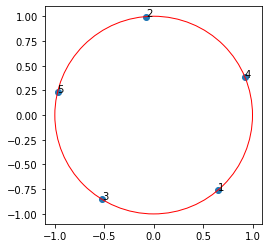
\includegraphics[scale=0.5]{maxcut-pentagon.png}
\end{center}

Resulta razonable elegir un conjunto $K$ tomando dos nodos vecinos en el gráfico.

\end{frame}

%------------------------------------------------------------------

\begin{frame}
\frametitle{Algoritmo Redondeo aleatorio de Goemans-Williamson}

En la situación general, tomamos un hiperplano que divida a la esfera unitaria en dos mitades y tomamos en $K$ a todos los nodos que quedan en una de estas dos mitades.

Más concretamente, para un vector aleatorio $\gb$ de norma 1, definimos
$$
K = \{i \in N: \inner{\gb}{\pb_i} \ge 0\}.
$$

Esto nos da un corte aleatorio, y podemos calcular la esperanza  del valor del corte (veremos más adelante cómo tomar un vector aleatorio).

\end{frame}

%------------------------------------------------------------------

\begin{frame}
\frametitle{Relación entre la relajación y el problema original}

La esperanza del valor del corte es
$$
E[w(\delta(K))] = E\left[\sum_{i  < j} w_{ij} \one_{(i,j) \in \delta(K)}\right] = \sum_{i < j} w_{ij} \Pr[(i,j) \in \delta(K)].
$$

Observamos que las probabilidades no son independientes, pero no es necesaria independencia para distribuir la esperanza con respecto a la suma.

\end{frame}

%------------------------------------------------------------------

\begin{frame}
\frametitle{Relación entre la relajación y el problema original}

Calculamos ahora $\Pr[(i,j) \in \delta(K)]$ para $(i,j)$ fijo.

Consideramos el plano que pasa por el origen y contiene a los dos vectores $\pb_i$ y $\pb_j$.
\begin{center}
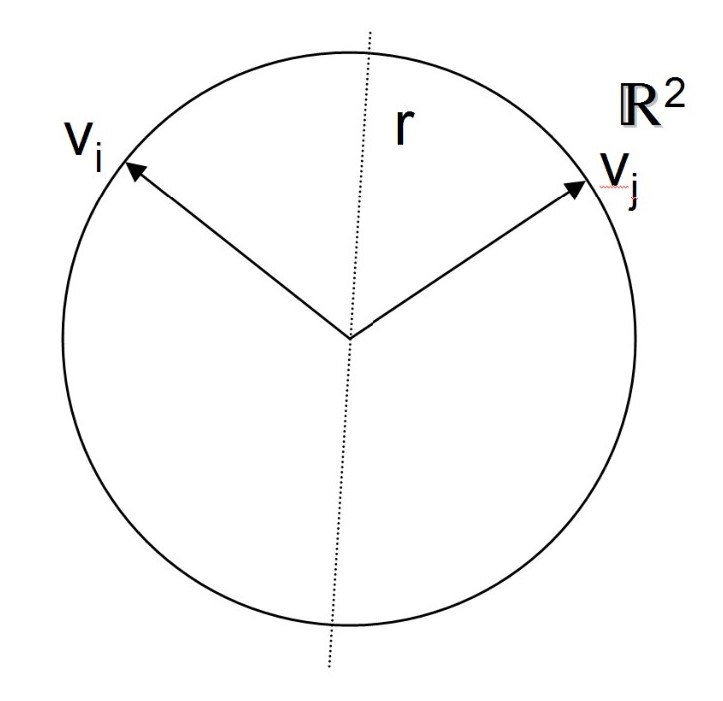
\includegraphics[scale=0.18]{maxcut-diameter.jpg}
\end{center}


La probabilidad de que un hiperplano separe a los dos vectores es la misma que la probabilidad de que un diámetro en este plano los separe.


\end{frame}

%------------------------------------------------------------------

\begin{frame}
\frametitle{Relación entre la relajación y el problema original}

Esta probabilidad es
$$
\Pr[(i,j) \in \delta(K)] = \frac{\angle(\pb_i, \pb_j)}{\pi} = \frac{\arccos(\inner{\pb_i}{\pb_j})}{\pi}.
$$


Por lo tanto, el valor esperado del corte es
$$
GW(K) = E[w(\delta(K))] = \sum_{i<j} w_{ij} \frac{\arccos(\inner{\pb_i}{\pb_j})}{\pi}.
$$


Llamamos $SDP(K)$ al valor óptimo del problema SDP correspondiente a la solución $\Xb = \Pb \Pb^T$.

Queremos comparar $E[w(\delta(K))]$ con este valor con $SDP(K)$.

%$$
%SDP(K) = \sum_{i,j} w_{ij} \left( \frac{1}{2} - \frac{1}{2} \inner{\pb_i}{\pb_j} \right) \ge OPT(K).
%$$

\end{frame}

%------------------------------------------------------------------

\begin{frame}
\frametitle{Relación entre la relajación y el problema original}

Recordemos que en la formulación original teníamos
$$
\xb^T \Cb \xb = w(\delta(K)) = \sum_{i < j}w_{ij}\frac{1-x_i x_j}{2}
$$
y tomando $\Xb = \xb \xb^T$ obtuvimos
$$
\innerTrace{\Cb}{\Xb} = w(\delta(K)) = \sum_{i < j}w_{ij}\frac{1-x_{ij}}{2}
$$
usando que $x_{ij} = x_i x_j$.

Por lo tanto, si tomamos $\Xb = \Pb^T \Pb$, las coordenadas de $\Xb$ son $x_{ij} = \inner{\pb_i}{\pb_j}$ y por lo tanto
$$
SDP(K) = \innerTrace{\Cb}{(\Pb^T\Pb)} = \sum_{i < j}w_{ij}\frac{1-\inner{\pb_i}{\pb_j}}{2}.
$$


\end{frame}

%------------------------------------------------------------------

\begin{frame}
\frametitle{Relación entre la relajación y el problema original}

Para comparar ambas expresiones término a término, consideramos
$$\rho = \pb_i \cdot \pb_j, \quad -1 \le \rho \le 1$$
y graficamos las funciones $f_1(\rho) = \frac{\arccos(\pb_i \cdot \pb_j)}{\pi}$ y $f_2(\rho)  = \frac{1}{2} - \frac{1}{2} (\pb_i \cdot \pb_j)$.

\begin{center}
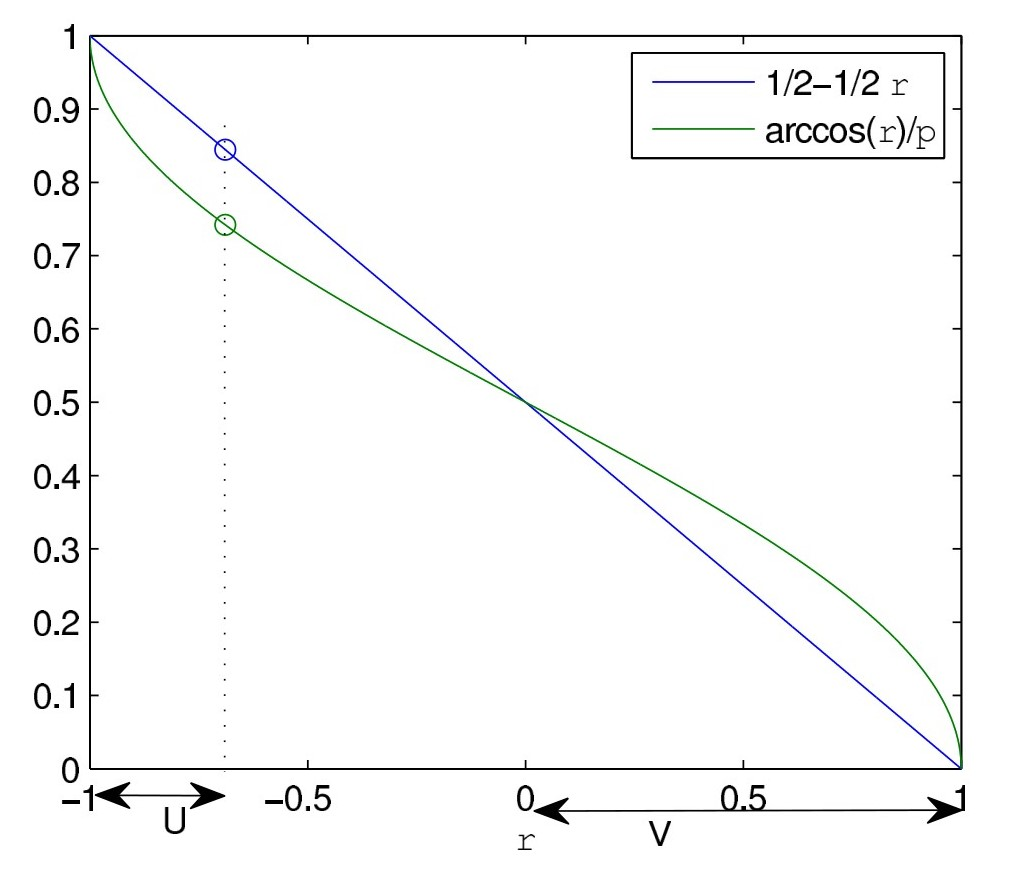
\includegraphics[scale=0.18]{maxcut-arccos.jpg}
\end{center}

\end{frame}

%------------------------------------------------------------------

\begin{frame}
\frametitle{Relación entre la relajación y el problema original}



Calculando la mayor diferencia entre las dos funciones, obtenemos que
$$f_1(\rho) \ge 0.87854 f_2(\rho)$$
y por lo tanto:
$$
GW(K) \ge 0.87854 \ SDP(K),
$$
y esto implica que existe algún corte $K^\star$ tal que $w(\delta(K^\star)) \ge 0.87854$ del valor óptimo del problema SDP.

Para el pentágono con todos los pesos de las aristas iguales a 1, la razón entre el valor óptimo del problema max-cut y la relajación SDP es aproximadamente $0.884$, por lo tanto la cota obtenida anteriormente esta cerca de la mejor cota que podemos obtener.

\end{frame}

%------------------------------------------------------------------

\end{document} 